\documentclass{article}
\usepackage{graphicx} % Required for inserting images
\usepackage{float}
\usepackage[T1]{fontenc}
\title{Analysing the Robustness of Deep Neural Networks}
\author{Divij Khaitan}
\date{\today}
\usepackage{amsmath}
\usepackage{amssymb}
\DeclareMathOperator{\softmax}{softmax}
\begin{document}

    \maketitle

    \section{Introduction}
        Deep Neural Networks have revolutionised several fields since it was discovered that they could be trained at scale on graphics processing units. Today, deeper and deeper networks trained on unfathomably large datasets are ubiquitous in everyday use, even for someone who may not be technically inclined. The increase in the sizes of neural networks does beg the question, how much is too big. Today, OpenAI's GPT-4 model has over a trillion parameters, even though the number of unique sentences it was trained was several orders of magnitude smaller. In practice it is observed that models do not appear to overfit their training data, a phenomenon that lacks an accepted explanation even today.
        
        The goal of this project is to provide a theoretical and practical analysis of the robustness properties of deep neural networks by analysing the patterns of neuron activations. 
        \subsection{Related work}
            
            \indent \textbf{Generalisation/Implicit Regularisation}: Zhang et. al. showed as early as 2017 that even AlexNet has enough capacity to fit all of imagenet with completely random labels perfectly when given enough time \cite{zhang2017understandingdeeplearningrequires}. This suggests that although networks have extremely high 'capacity', they do not use all of it in practice and that contrary to statistical wisdom, they are not overfitting as a result of overparameterisation. Arora et. al. showed that overparameterisation provides a speed up to the optimisation of neural networks and provided bounds for the generalisation error of two layer ReLU networks \cite{pmlr-v80-arora18a}. Soltanolkotabi and Oymak showed that networks that polynomially overparameterised in the size of the input are resistant to label corrpution, with the final parameters being close to their initialised values \cite{pmlr-v108-li20j}. A major hypothesis in this area is that stochastic gradient descent(SGD) as a training method introduces an 'implicit regularisation' into the training of a deep network. Norm minimisation was one explanation for this behaviour, first put forth by \cite{neyshabur2015searchrealinductivebias}. Several notions of complexity have been put forth, including VC dimension and Rademacher complexity, see \cite{neyshabur2017implicitregularizationdeeplearning} for a more granular view of these. Examples where all matrix norms diverge were constructed in \cite{razin2020implicitregularizationdeeplearning}, indicating that the relationship between weight decay and implicit regularisation requires more inspection. This relationship has also been questioned by \cite{arora2019implicitregularizationdeepmatrix}, which shows that for the case of matrix factorisation, matrix norms are insufficient to describe the action of gradient-based optimisation. This paper also shows that adding depth to matrix factorisation encourages low rank solutions, which improve the accuracy of the reconstruction. \cite{gissin2019implicitbiasdepthincremental} formally showed that deep networks learn 'incrementally', and while shallow networks can exhibit similar behaviour they do so for a small set of initial conditions. \cite{arpit2017closerlookmemorizationdeep} showed that SGD behaves differently on noise as opposed to actual datasets, and that dropout works better than noise injection for hindering memorisation while promoting generalisation

            \textbf{Out of Distribution Detection}: When considering open world deployment of networks, it simply isn't possible to train them on exhaustive partition of every input they can expect. Thus, it becomes important to develop mechanisms that allow users to detect when an input is outside the training distribution of a model. The first major work that tackled this problem with some effectiveness was \cite{hendrycks2018baselinedetectingmisclassifiedoutofdistribution}, which uses $-\max_i \softmax(f(x)_i)$ as a means of detecting if a particular input is outside the training distribution. This is analogous to treating the magnitude of the softmax output as a confidence measure, which isn't entirely accurate as pointed out by the authors. However, this has proven to be a baseline which is difficult to beat non-trivially. \cite{hendrycks2019deepanomalydetectionoutlier} describes a method for fine-tuning trained models to detect OOD inputs using unlabelled data and the KL divergence from a uniform distribution. ODIN \cite{liang2020enhancingreliabilityoutofdistributionimage} has empirically shown excellent performance on OOD detection, but requires tuning hyperparameters beforehand. \cite{lee2018simpleunifiedframeworkdetecting} Uses a similar idea of creating a probability distribution over feature spaces and uses the minimum mahalanobis distance as a classifier, and also use it to show that tuning their classifier on certain adversarial attacks adds robustness to other adversarial attacks. The authors assume a multivariate gaussian distribution on the class-conditional softmax probability vectors, and for a vector output the class for which the probability vector has the smallest mahalanobis distance. \cite{sastry2020detectingoutofdistributionexamplesindistribution} Uses the gram matrices of the feature vectors and computes layer-wise deviations of an input from the normal values of the class.
            % TODO: Concept and Covariate Shift, add and explain literature

            \textbf{Activation Patterns of Neural Networks}: There has been some past work on analysing the patterns of activation of neural networks. On the side of interpretability, SUMMIT (citation) and NAP (citation) both attempt to identify 'important' neurons in an attempt to interpret the features associated with different classes. Similar ideas have been used for the detection of rare classes as well as the detection of misclassifications at test-time. Our work is more similar to the latter, however we take a different approach to analysing the patterns.  

            \textbf{Adversarial Robustness}: Szegdy et. al. discovered \cite{szegedy2014intriguingpropertiesneuralnetworks} in 2014 that classifiers on vision models are susceptible to extremely small changes (in some $L^p$ space) that can cause a misclassfification. Since then, a considerable amount of work has gone into attempting to explain their existence (\cite{shafahi2020adversarialexamplesinevitable}, \cite{shamir2022dimpledmanifoldmodeladversarial}) and the development of attacks (PGD \cite{madry2019deeplearningmodelsresistant}, FGSM\cite{goodfellow2015explainingharnessingadversarialexamples}) and defenses to those attacks, either by changing the loss function or by modifying the training algorithm in some way. 
            
            \textbf{Manifold Hypothesis}: This is an idea that pre-dates deep learning, that most real-world datasets in high dimensions have an underlying low dimensional structure. In the context of machine learning, it has primarily been studied from the perspective of dimensionality reduction, reducing a set of points in a high dimensional space to one in a low dimensiona space which is equivalent to it. \cite{fefferman2013testingmanifoldhypothesis} develops an algorithm to test the hypothesis, and \cite{NIPS2010_8a1e808b} discusses the sample complexity of the problem. See \cite{meil2023manifoldlearningwhathow} for a survey of the most recent methods in the field. 

            % \textbf{Lottery Ticket Hypothesis}: The sparsity of activations in neural networks is widely seen in practice. Frankle and Carbin suggested that a small subset of neurons are better primed to fit the dataset at initialisation time, and dubbed this the 'lottery ticket hypothesis'. Subsequent work has focused on algorithms for identifying such lottery tickets. 

    \section{Methods}
        % Shifts in distribution are situation when the distributions of the training and testing sets are not identical. In literature, the most common classification of these shifts are concept shift and covariate/data shift.

        % \textbf{Covariate Shift} is when $p(x)$ changes, but not $p(y|x)$, i.e. the inputs change but the labels stay the same. An example would include training a model on voting patterns for India, and testing the model on voting patterns from China.
        
        % \textbf{Concept Shift} is when $p(x)$ remains the same, but $p(y | x)$ does not. This can be thought of as training on a similar dataset with slightly different labels. An example would be training a model to issue red alerts for storms in Delhi, and testing it to issue red alerts in Pune. While both cities might see similar rainfall patterns, they may be equipped very differently to handle the same amount of precipitation. 

        % Detecting such shifts can be difficult in practice, because the distributions themselves cannot be characterised easily. Our hypothesis is that in CNNs, the neurons from the fully connected layers should have similar activation patterns across the same classes, and thus we should be able to attach distributions of neuron activations to each class, which should be sensitive to a shift in the distribution of inputs. 
        
    % \section{Class-wise Frequencies of Neuron Activations}
    %     For this section, we analysed the outputs of each fully connected hidden layer, i.e. for a network $f = \phi_{n}(f_{n}(\dots(\phi(f_1(x)))))$, we analysed $x_k = \phi(f_{k}(\dots(\phi(f_1(x)))))$. Alexnet in particular is RELU-activated with the exception of the final layer, so $\phi_i = \text{ReLU} \text{ if } i < n \; \sigma(x) \text{ if } i = n$. We utilised the following definitions of significance \\
    %     \[S_1(x_{i}) = 1 \text{ if } x_i > 0\] 
    %     \[S_2(x_{(i)}) = 1 \text{ if } \frac{x_{(i)}}{x_{i+1}} > \epsilon\] 
    %     $x_{(i)}$ denotes the i$^\text{th}$ order statistic. The first definition is comes from the ReLU activation, where a neuron is considered 'active' if it is positive. The justification for the second is the assumption of a high signal to noise ratio, where smaller activations correspond to noise while larger activations correspond to meaningful information. Practically, we set the value of $\epsilon$ to be 1000. We computed the proportions of every neuron activating in any given class under both definition, and the results are attached below. Each neuron has a proportion of activations for each class in between 0 and 1, we have displayed histograms of the number of neurons in 100 bins for different activation proportions. Below is the result for a particular class under both $S_1$ and $S_2$. The y-axis is the number of neurons in each bin, and the x-axis has the bins of different proportions of activation across all the images in the class. This shows a move towards sparsity in activation with an increase in depth.
    %     \begin{figure}[H]
    %         \centering
    %         \begin{minipage}{0.45\textwidth}
    %             \centering
    %             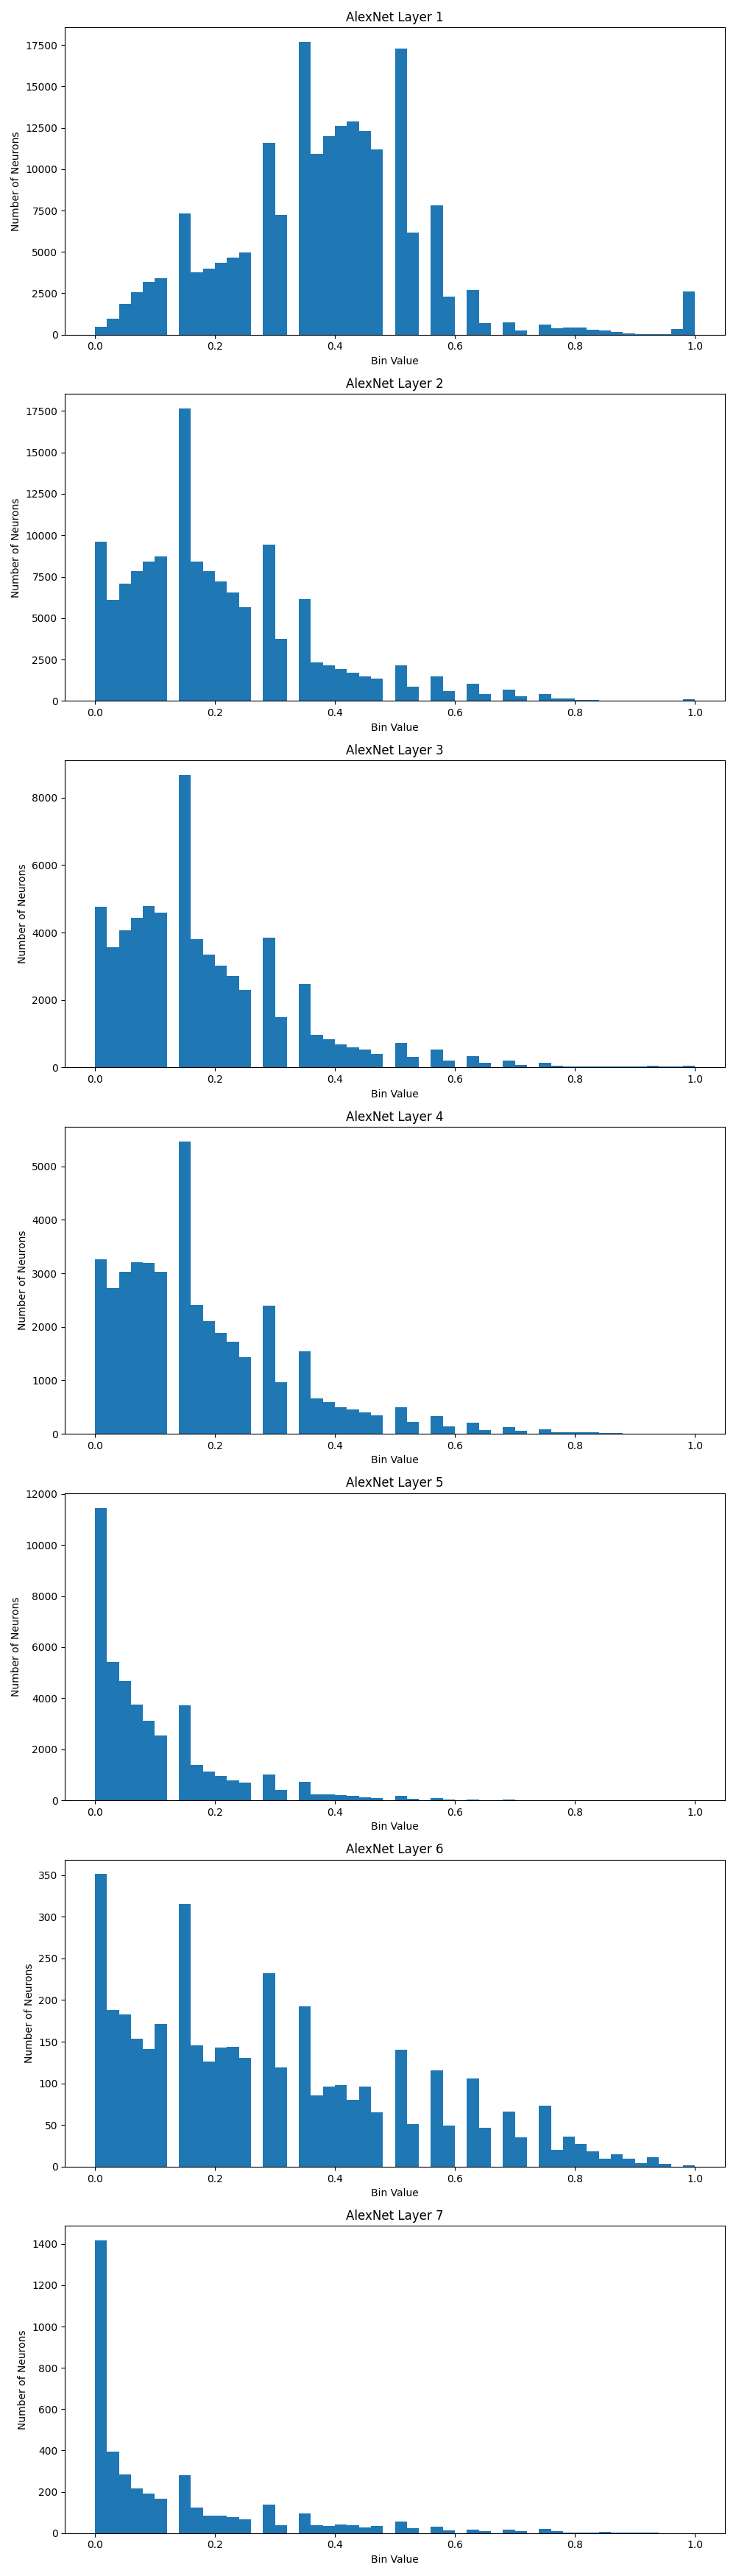
\includegraphics[width=\textwidth]{images/alexnet_class_frequency_list_n01601694.png}
                
    %         \end{minipage}\hfill
    %         \begin{minipage}{0.45\textwidth}
    %             \centering
    %             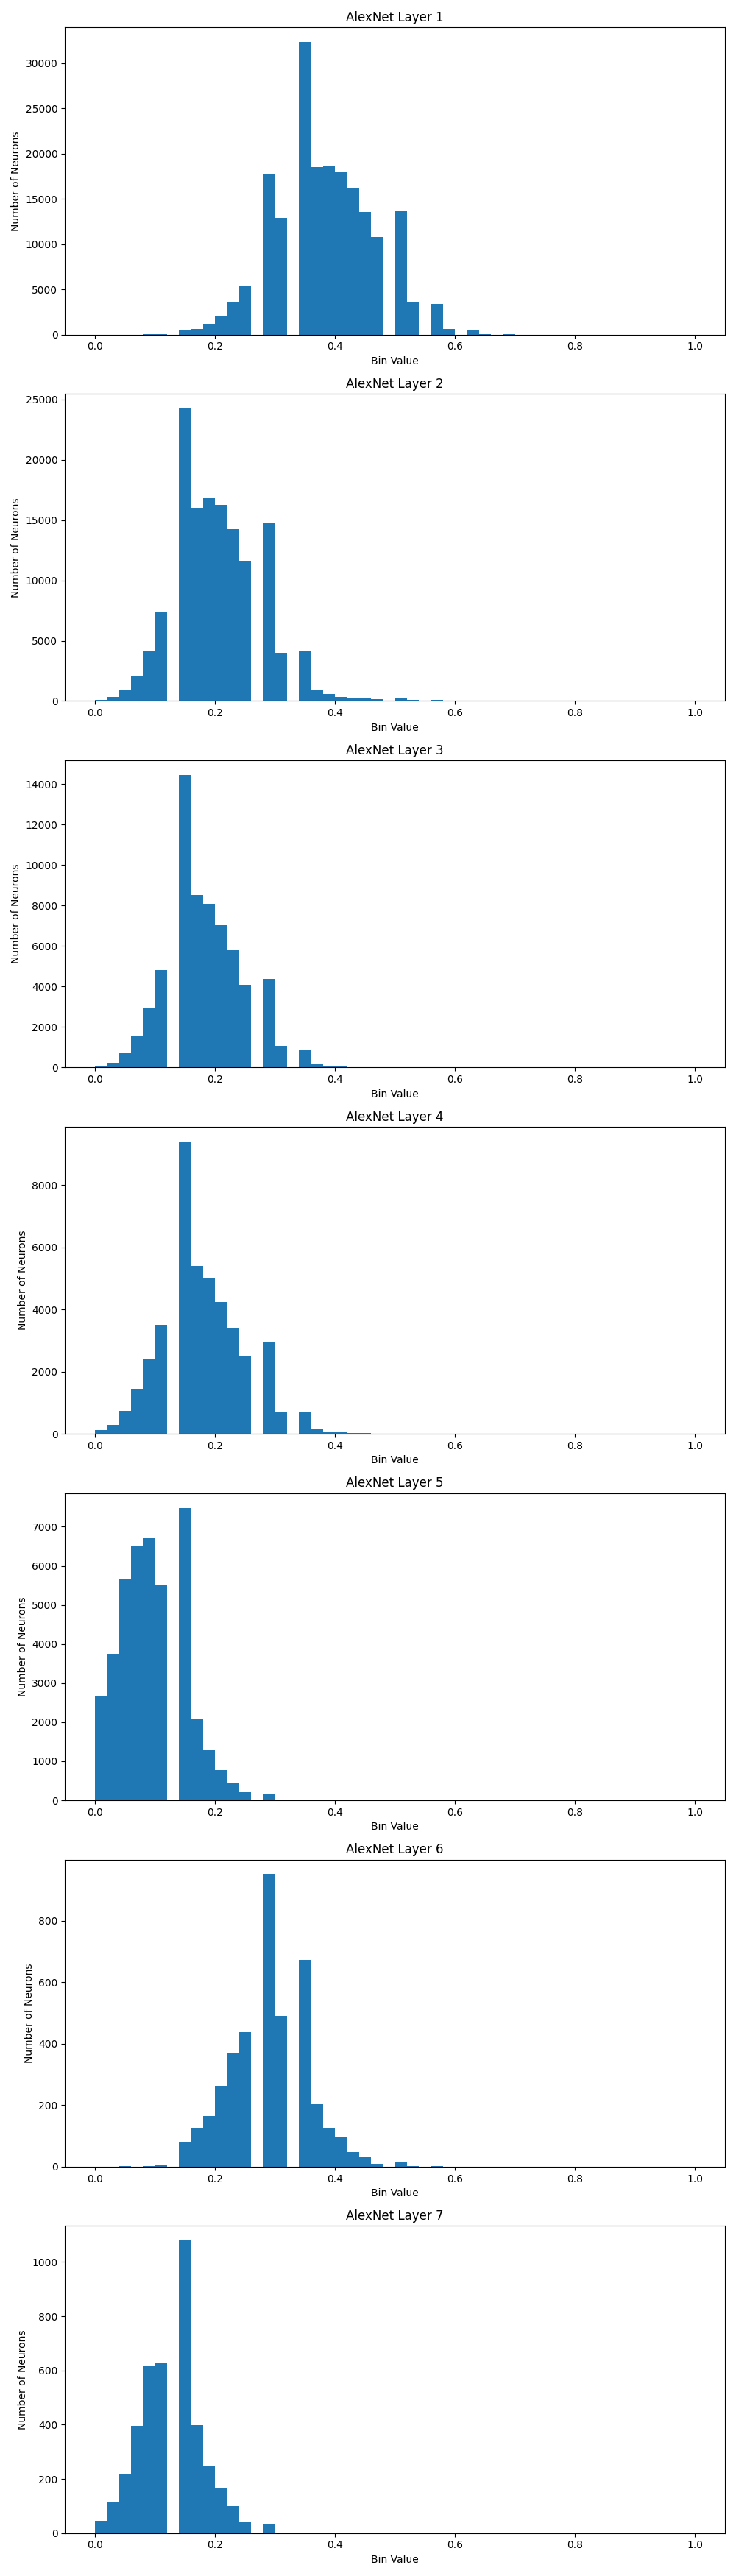
\includegraphics[width=\textwidth]{images/alexnet_class_frequency_list_threshold_n01601694.png}
    %         \end{minipage}
    %         \caption{Histograms for AlexNet activations under $S_1$(left) and $S_2$(right). There is a distinct clustering towards the left inside the convolutional layers (plots 1 to 5) and then inside the fully connected layers as well (plots 6 and 7)}
    %         \label{fig:neuron_activation_frequency}
    %     \end{figure}

    %     % \begin{figure}[ht]
    %     %     \centering
    %     %     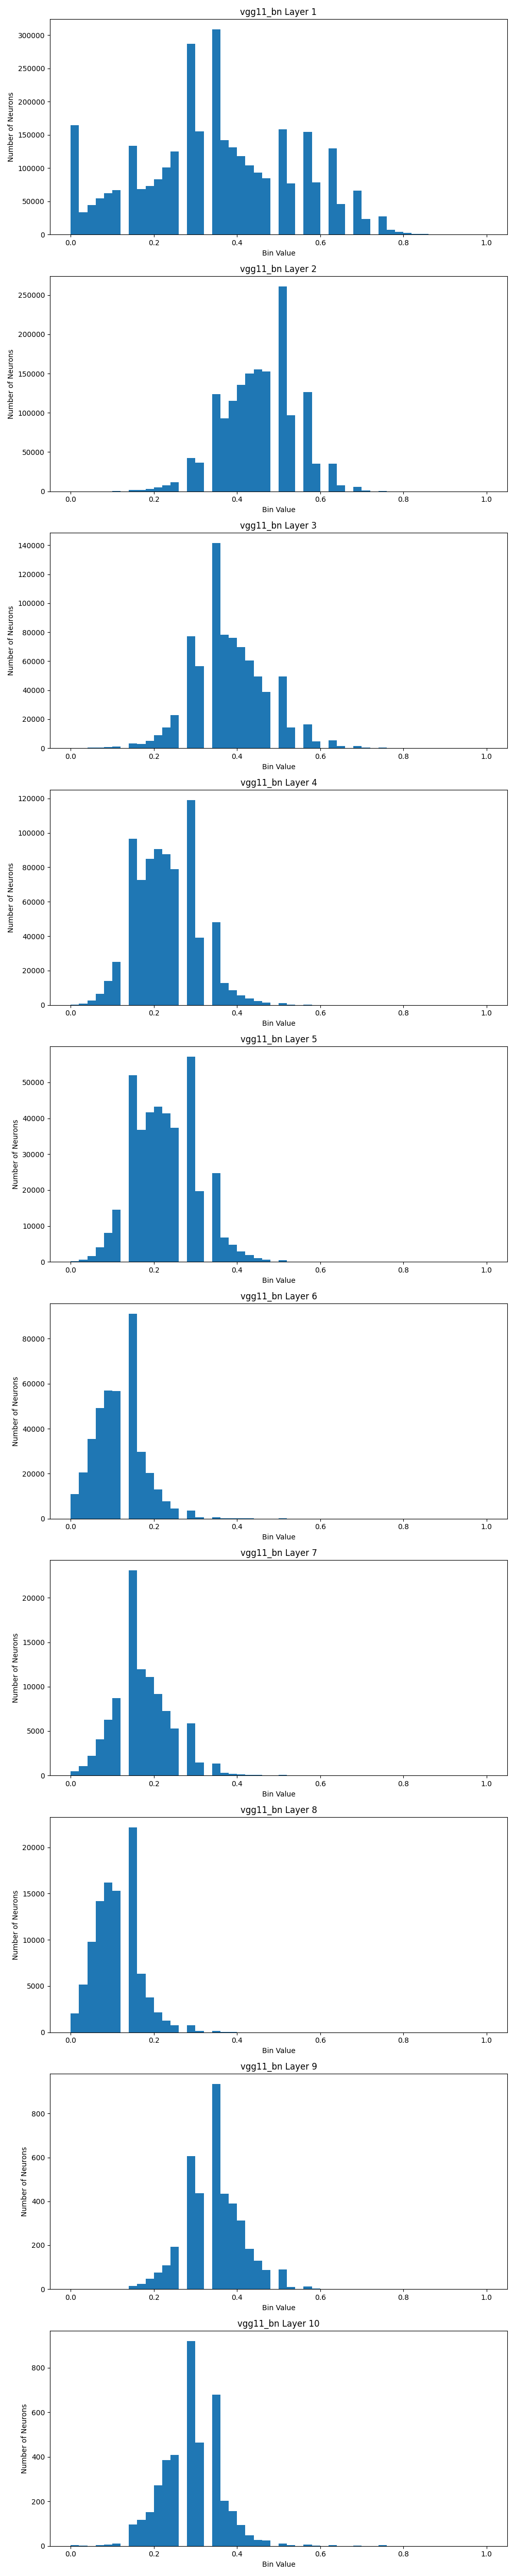
\includegraphics[height=\textheight,keepaspectratio]{vgg11_bn_class_frequency_list_n01601694.png}
    %     %     \caption{Histogram for VGG11 with thresholding. We observe the same behaviour here}
    %     %     \label{fig2}
    %     % \end{figure}
    % \section{Class-wise Patterns of Neuron Activations}
    %     We also plotted the proportion of successes of each neuron in each layer. Some of the results for the final layer of different classes are attached below. The key takeaway is once again the sparsity of the activations, with most neurons having small activations and a few neurons having large activations. For ease of viewing, the vectors were ravelled to form a rectangle with approximately equal sides. Below attached are results from the final 2 layers of a single class.
    %     \begin{figure}[H]
    %         \centering
    %         \begin{minipage}{0.45\textwidth}
    %             \centering
    %             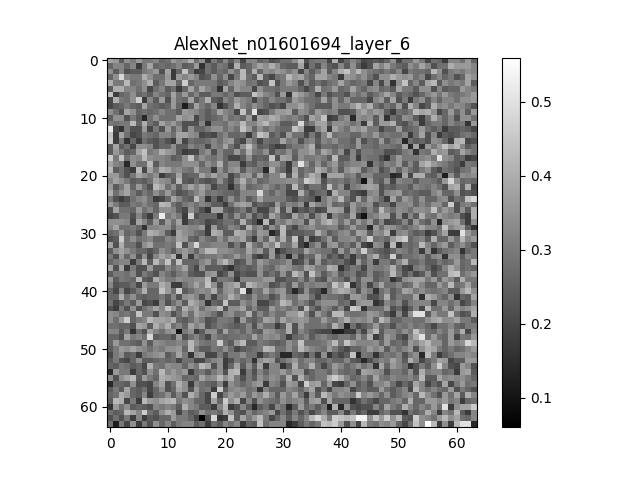
\includegraphics[width=\textwidth]{images/AlexNet_n01601694_layer_6.png}
                
    %         \end{minipage}\hfill
    %         \begin{minipage}{0.45\textwidth}
    %             \centering
    %             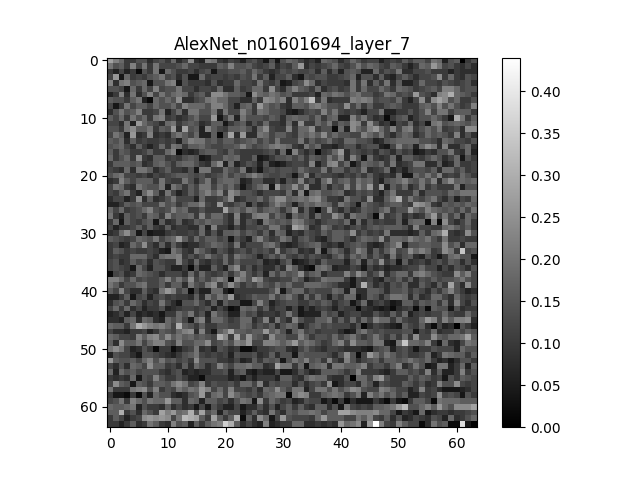
\includegraphics[width=\textwidth]{images/AlexNet_n01601694_layer_7.png}
    %         \end{minipage}
    %         \caption{Activation proportions of neurons for the fully connected layers 6 and 7 of alexnet}
    %         \label{fig:neuron_activation_pattern}
    %     \end{figure}
        
    % \section{Entropies in Between Classes}
        
        \subsection{Class-Wise Frequencies of Significant Neuron-Weight Interactions}
            As an additional approach, we decided to study the interactions in a neural network at a more granular level. Instead of just looking at the final value of the neuron, we decided to look at each individual weight being multiplied into each neuron. In this case, what we did is described below. 

            The final layer of the neural network operates as follows. Given an activation vector $x \in \mathbb{R}^{n_{in} \times 1}$ and a weight matrix $W \in \mathbb{R}^{n_{out} \times n_{in}}$ 
                \[
                    \begin{bmatrix}
                        w_{1,1} & \dots & w_{1,n_{in}} \\
                        \vdots & \ddots & \vdots \\
                        w_{n_{out}, 1} & \cdots & w_{n_{out}, n_{in}} \\
                    \end{bmatrix}
                    \begin{bmatrix}
                        x_1 \\
                        \vdots \\
                        x_{n_{in}} \\
                    \end{bmatrix}
                    = 
                    \begin{bmatrix}
                        w_{1,1}x_1 + w_{1, 2}x_2 + \dots + w_{1, n_{in}}x_{n_{in}} \\
                        \vdots \\
                        w_{n_{out},1}x_1 + w_{n_{out}, 2}x_2 + \dots + w_{n_{out}, n_{in}}x_{n_{in}}
                    \end{bmatrix}
                \]
                This would not allow us to study the individual activation-weight pairs, because they would all be summed up. A vector operation that computes the sum over the rows of a matrix is postmultiplication by the all 1s vector, so by factoring out this vector we can get the required information. Factoring out the all 1s vector from the neurons in the penultimate layer, we get an diagonal matrix with the neurons activations as entries 
                \[
                    \begin{bmatrix}
                        w_{1,1} & \dots & w_{1,n_{in}} \\
                        \vdots & \ddots & \vdots \\
                        w_{n_{out}, 1} & \cdots & w_{n_{out}, n_{in}} \\
                    \end{bmatrix}
                    \begin{bmatrix}
                        x_1  & \dots & 0 \\
                        \vdots & \ddots & \vdots \\
                        0 & \dots & x_{n_{in}} \\
                    \end{bmatrix}
                    = 
                    \begin{bmatrix}
                        w_{1,1}x_1  & \dots & w_{1,n_{in}}x_1 \\
                        \vdots & \ddots & \vdots \\
                        w_{n_{out}, 1}x_{n_{in}} & \dots & w_{n_{out}, n_{in}}x_{n_{in}} 
                    \end{bmatrix}\]
            To this, we concatenated the bias vector as an additional neuron, giving us a matrix in $\mathbb{R}^{n_{out} \times (n_{in} + 1)}$
            The definition of significance we decided on was 
            \[S(x_{ij}) = 1 \text{ if } \frac{x_{ij}}{\sum_j x_{ij}} > \frac{1}{n_{in}} \]
            where $n_{in}$ is the number of input features, i.e. number of columns in the matrix. The justification behind this is the idea that if an activation is of an above average proportion of the final activation, the neuron-weight interaction is significant.
            As eariler, we hypothesise that the number of significant interactions between neurons and weights are sparse, and that the sparsity increases with depth. To this end, we attempted to bin the proportions of the significance of each neuron-weight interaction. If the activations become more sparse, the number should be larger on the left and become sparse towards the end, which should be exacerbated by depth. 
            
        \subsection{KL Divergence Between Classes}
            Building on the same experiment, we wanted to check both the entropies in between different classes over the activation distribution for the same layer. We also measured the same entropies at training and testing time, as well as an in and out of distribution dataset. The in-distribution dataset was the validation set for imagenet as used eariler, and the out of distribution dataset was fixed to be the imagenet-r dataset created by Hendrycks et. al.\cite{hendrycks2021facesrobustnesscriticalanalysis}. This is a collection of stylised versions of the standard classes of imagenet such as caricatures. This dataset has 200 classes compared to the original 1000 from imagenet, and to ensure the comparison was meaningful we sampled 50 classes from the dataset uniformly at random and computed the pairwise KL divergences between pairs of classes from the imagenet validation set, between pairs of classes from the imagenet-r set and between the same classes from imagenet and imagenet-r. Along similar lines, we also measured the entropy of the distributions. Analagous to regression, the distance within the clusters(entropy) should decrease, while the distance between the clusters(KL-divergence) should increase. The entropy is given by the formula
            \[H(X) = -\sum p(x)\log(p(x))\]
            Where $p(x)$ is the probability that the random variable $X$ takes on the value $X$. Intuitively, it is a measure of 'disorder' in the random variable. The KL divergence is the relative entropy between 2 distributions, given by the formula 
            \[D_{KL}(P||Q) = \sum P(x)\log(\frac{P(x)}{Q(x)})\]
            This can be thought of as a measure of how well $P$ approximates $Q$. It is not a true metric, because it doesn't satisfy triangle inequality or symmetry. Our computations make a strong assumption of \textbf{independence} of the significance of activations, i.e. that any activation will be significant in it's own row is independent of the other events being significant. 
        
        \subsection{Memorisation and Significance}
            We hypothesise that a network which has memorised it's training data would have significantly different properties in terms of sparsity and the separation of classes. To this end, we replicate the experiment specified in \cite{zhang2017understandingdeeplearningrequires} and train a modified version of AlexNet on CIFAR10 until it reaches zero error. The details of the training stay the same and will be provided in Appendix A. 
        
        \subsection{Adversarial Attacks}
            The above gives us a distribution on the activations for a given class. We compared the probabilities conditioned on the distribution of the class of the validation images subject when subjected to a PGD attack \cite{madry2019deeplearningmodelsresistant}. The parameters of the attack are given in Appendix B. 
        
        \subsection{Manifold Entaglement}
            In the $n-1^{th}$ hidden layer, the manifolds for different classes should be linearly separable. This is because the following transformations are an affine hidden layer computation and a linear softmax computation. We estimate the dimensionality of the manifolds spanned by each class by inspecting the neurons for this layer, combining them into a matrix and finding it's rank. We further estimate the degree of overlap between the manifolds by combining the matrices for different classes and then applying the principle of inclusion and exclusion. Networks that have not overfit their training data should have manifolds with little overlap, while those which have should have entagled class manifolds. We additionally expect the manifolds to have smaller dimensionality for networks with better embeddings. 

    \section{Results}
        We examined the distributions for AlexNet, VGG, ResNet and InceptionV3. The experiments were run using PyTorch, and the weights for the pretrained versions of the networks were also taken from there. The datasets used was the validation set for Imagenet \cite{russakovsky2015imagenetlargescalevisual}, and CIFAR10 \cite{Krizhevsky2009LearningML}
        \subsection{Sparsity of Activations}
            The following plots have the number of times a neuron activated over the entire validation set divided by the length of the validation set on the x axis, and the y-axis is the number of neurons that activate in that 'bin', divided by the total number of neurons.
            The results indicate that training encourages sparsity quite strongly, with the proportions of neurons that are always on dropping from 0.2 and 0.1 to 0.05 and $<$ 0.01 on the last and second last layers respectively from the untrained model to the best model. The network fitting random labels has an extremely sparse penultimate layer, with the best network having some density to it and the overtrained network resembling a mid-point in between the random labelled and the best network. 
            
            \begin{figure}[H]
                \centering
                \begin{minipage}{0.45\textwidth}
                    \centering
                    \includegraphics[width=\linewidth]{new/small_alexnet_untrained_cifar10/activation_proportions/cy_list_0.png}
                    \caption{Untrained}
                    % \label{fig:image1}
                \end{minipage}
                \hfill
                \begin{minipage}{0.45\textwidth}
                    \centering
                    \includegraphics[width=\linewidth]{new/small_alexnet_cifar10_random_labels/activation_proportions/cy_list_0.png}
                    \caption{Random Labels}
                    % \label{fig:image2}
                \end{minipage}
                \begin{minipage}{0.45\textwidth}
                    \centering
                    \includegraphics[width=\linewidth]{new/small_alexnet_cifar10_250_epoch/activation_proportions/cy_list_0.png}
                    \caption{Overtrained}
                    % \label{fig:image1}
                \end{minipage}
                \hfill
                \begin{minipage}{0.45\textwidth}
                    \centering
                    \includegraphics[width=\linewidth]{new/small_alexnet_cifar10_best/activation_proportions/cy_list_0.png}
                    \caption{Best}
                    % \label{fig:image2}
                \end{minipage}
                \hfill
                
                \caption{Activation Proportions from the class Airplane on (from left to right) the last and second last layers for the random labels and the last and second last layers clean labels respectively}
                \label{fig:class_airplane}
            \end{figure}
            
            \begin{figure}[H]
                \centering
                \begin{minipage}{0.45\textwidth}
                    \centering
                    \includegraphics[width=\linewidth]{new/small_alexnet_untrained_cifar10/activation_proportions/cy_list_7.png}
                    \caption{Untrained}
                    % \label{fig:image1}
                \end{minipage}
                \hfill
                \begin{minipage}{0.45\textwidth}
                    \centering
                    \includegraphics[width=\linewidth]{new/small_alexnet_cifar10_random_labels/activation_proportions/cy_list_7.png}
                    \caption{Random Labels}
                    % \label{fig:image2}
                \end{minipage}
                \begin{minipage}{0.45\textwidth}
                    \centering
                    \includegraphics[width=\linewidth]{new/small_alexnet_cifar10_250_epoch/activation_proportions/cy_list_7.png}
                    \caption{Overtrained}
                    % \label{fig:image1}
                \end{minipage}
                \hfill
                \begin{minipage}{0.45\textwidth}
                    \centering
                    \includegraphics[width=\linewidth]{new/small_alexnet_cifar10_best/activation_proportions/cy_list_7.png}
                    \caption{Best}
                    % \label{fig:image2}
                \end{minipage}
                \hfill
                
                % \caption{Activation Proportions from the class Frog on (from left to right) the last and second last layers for the random labels and the last and second last layers clean labels respectively}
                \label{fig:class_frog}
            \end{figure}
            Below are the results for the last 3 layers of alexnet on imagenet and imagenet-r, both trained and untrained. For AlexNet, we can see that the randomly initialised network looks the same in terms of activation proportions for all the layers across both datasets as expected. We once again see that training encourages sparsity in the network, even on the out of distribution set. While both classes are indistinguishable on the final and third-last layers, the in-distribution dataset is sparser on the final layer and the penultimate layer. In fact, there is a significant increase in the proportion of stray activations on the out of distribution dataset, suggesting that sparsity may be a characteristic of the neuron activations. 
            \begin{figure}[H]
                \centering
                \begin{minipage}{\textwidth}
                    \centering
                    \includegraphics[width=\textwidth]{new/alexnet_untrained_imgr_out/activation_proportions/n02088466.png}
                    
                \end{minipage}\hfill
                \begin{minipage}{\textwidth}
                    \centering
                    \includegraphics[width=\textwidth]{new/alexnet_imgr_out/activation_proportions/n02088466.png}
                \end{minipage}
                \begin{minipage}{\textwidth}
                    \centering
                    \includegraphics[width=\textwidth]{new/alexnet_untrained_r/activation_proportions/n02088466.png}
                    
                \end{minipage}\hfill
                \begin{minipage}{\textwidth}
                    \centering
                    \includegraphics[width=\textwidth]{new/alexnet_r/activation_proportions/n02088466.png}
                \end{minipage}
                
                \caption{Frequencies of the significant neuron-weight activation proportions for a single class top: untrained on imagenet, second: trained on imagenet, third: untrained on imagenet-r, bottom: trained on imagenet-r}
                \label{fig:frequency_neuron_weight1}
            \end{figure}
            
            % \begin{figure}[H]
            %     \centering
            %     \begin{minipage}{\textwidth}
            %         \centering
            %         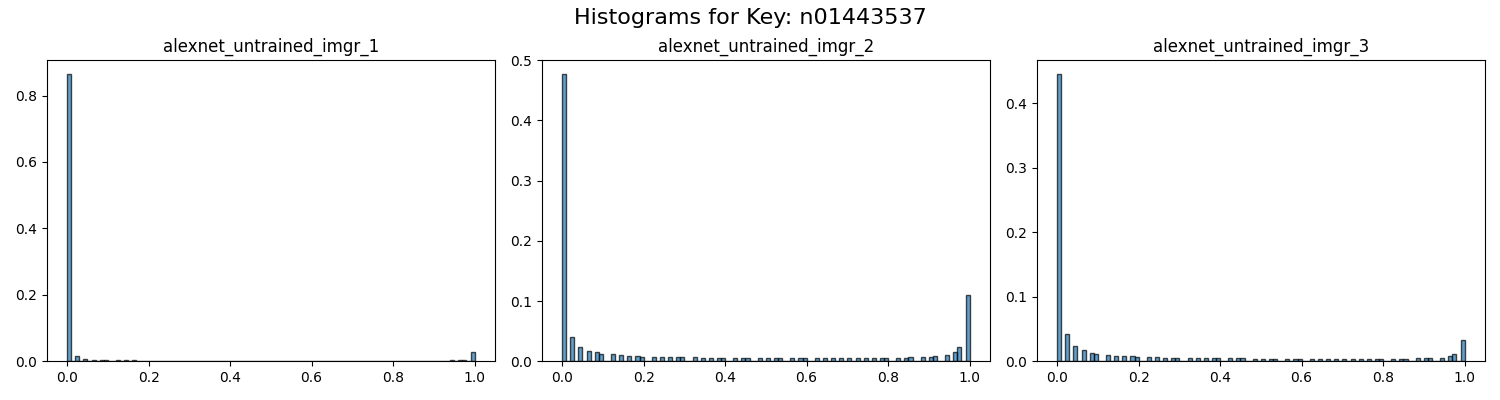
\includegraphics[width=\textwidth]{new/alexnet_/alexnet_untrained_imgr_n01443537.png}
                    
            %     \end{minipage}\hfill
            %     \begin{minipage}{\textwidth}
            %         \centering
            %         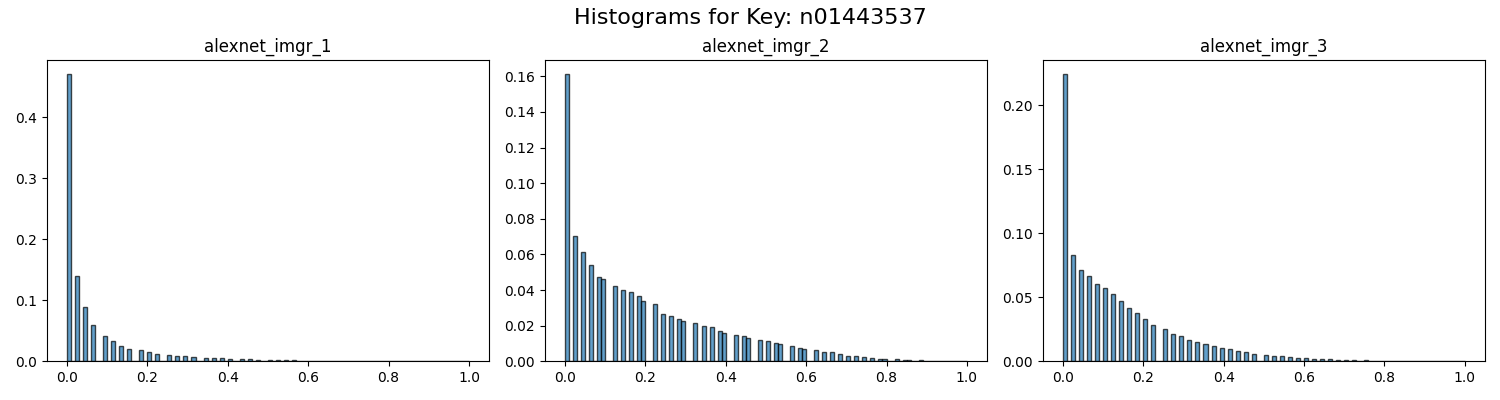
\includegraphics[width=\textwidth]{new/alexnet_/alexnet_imgr_n01443537.png}
            %     \end{minipage}
            %     \begin{minipage}{\textwidth}
            %         \centering
            %         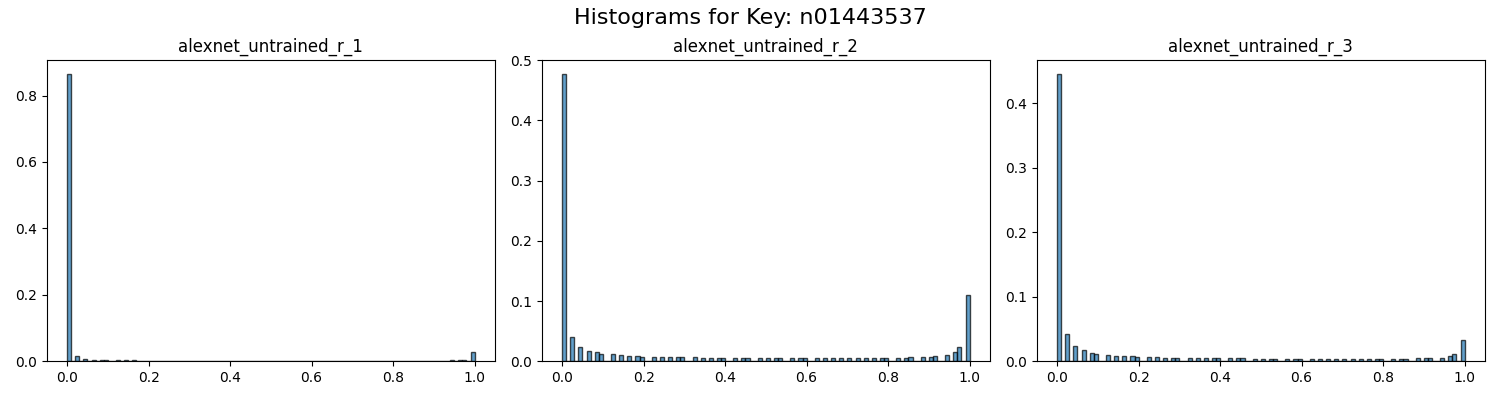
\includegraphics[width=\textwidth]{new/alexnet_/alexnet_untrained_r_n01443537.png}
                    
            %     \end{minipage}\hfill
            %     \begin{minipage}{\textwidth}
            %         \centering
            %         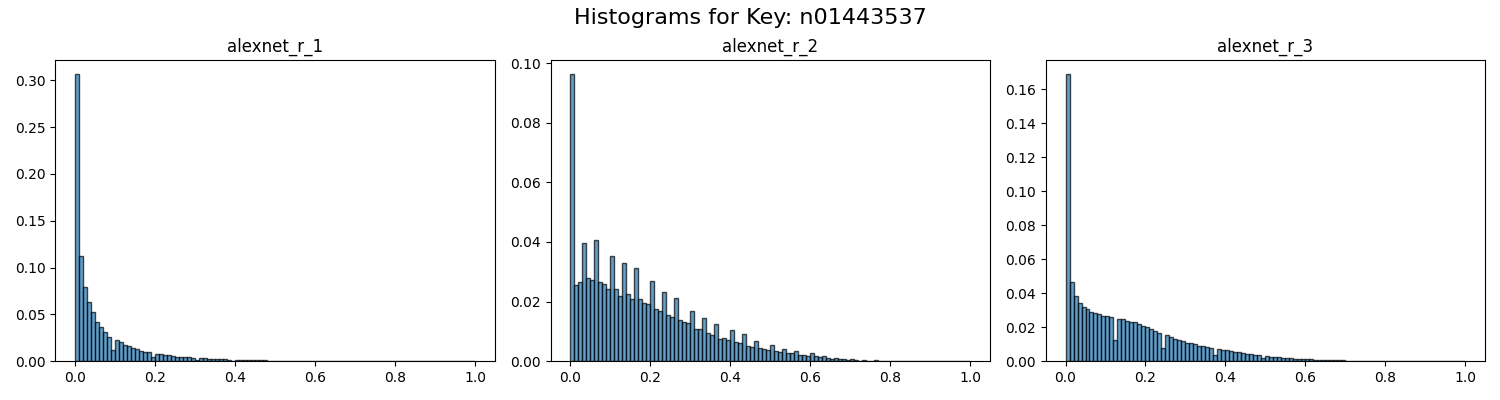
\includegraphics[width=\textwidth]{new/alexnet_/alexnet_r_n01443537.png}
            %     \end{minipage}
                
            %     \caption{Frequencies of the significant neuron-weight activation proportions for a single class top: untrained on imagenet, second: trained on imagenet, third: untrained on imagenet-r, bottom: trained on imagenet-r}
            %     \label{fig:frequency_neuron_weight2}
            % \end{figure}
    
    
    % \section{Patterns of Activation in Neuron-Weight Interactions}

        \subsection{Divergences of Neuron Weight Interactions}
            Below are the results for the KL-divergences of alexnet normalised corrected for the dimensionality of the space. Each row represents the KL divergence from a class, while a column represents the KL divergences to a class. The values on the diagonals for KL divergence would have been 0 and we plot the entropy of the distribution for that class instead.  Between initialisation and the end of training on the in-distribution dataset, we see that the separation of classes increases greatly, while the entropy of the class distributions decreases simultneously. This decrease is much more noticable at the deeper layers of the network, and also extremely telling between the networks for the in-distribution classes and out of distribution classes. The OOD classes become more separated from each other but their entropies see no decrease after training is complete, even seeing significant increases in some cases. 
            % KL Matrix In Distribution
            \begin{figure}[H]
                \centering
                \begin{minipage}{0.45\textwidth}
                    \centering
                    \includegraphics[width=\textwidth]{new/alexnet_untrained_imgr_out/out_matrices/alexnet_kl_matrix.png}
                    
                \end{minipage}\hfill
                \begin{minipage}{0.45\textwidth}
                    \centering
                    \includegraphics[width=\textwidth]{new/alexnet_imgr_out/out_matrices/alexnet_kl_matrix.png}
                \end{minipage}
                \begin{minipage}{0.45\textwidth}
                    \centering
                    \includegraphics[width=\textwidth]{new/alexnet_untrained_imgr_out_second_last/out_matrices/alexnet_kl_matrix.png}
                    
                \end{minipage}\hfill
                \begin{minipage}{0.45\textwidth}
                    \centering
                    \includegraphics[width=\textwidth]{new/alexnet_imgr_out_second_last/out_matrices/alexnet_kl_matrix.png}
                \end{minipage}
                
                \begin{minipage}{0.45\textwidth}
                    \centering
                    \includegraphics[width=\textwidth]{new/alexnet_untrained_imgr_out_third_last/out_matrices/alexnet_kl_matrix.png}
                    
                \end{minipage}\hfill
                \begin{minipage}{0.45\textwidth}
                    \centering
                    \includegraphics[width=\textwidth]{new/alexnet_imgr_out_third_last/out_matrices/alexnet_kl_matrix.png}
                \end{minipage}
                
                \caption{KL divergences between different classes for the untrained(left) and trained(right) classes of alexnet on imagenet. From top to bottom, these are the values for the distributions for the last, second last and third last layers}
                \label{fig:kl_divergences_imgr}
            \end{figure}
            
            % KL Matrix Out of Distribution
            \begin{figure}[H]
                \centering
                \begin{minipage}{0.45\textwidth}
                    \centering
                    \includegraphics[width=\textwidth]{new/alexnet_untrained_r/out_matrices/alexnet_kl_matrix.png}
                    
                \end{minipage}\hfill
                \begin{minipage}{0.45\textwidth}
                    \centering
                    \includegraphics[width=\textwidth]{new/alexnet_r/out_matrices/alexnet_kl_matrix.png}
                \end{minipage}
                \begin{minipage}{0.45\textwidth}
                    \centering
                    \includegraphics[width=\textwidth]{new/alexnet_untrained_r_second_last/out_matrices/alexnet_kl_matrix.png}
                    
                \end{minipage}\hfill
                \begin{minipage}{0.45\textwidth}
                    \centering
                    \includegraphics[width=\textwidth]{new/alexnet_r_second_last/out_matrices/alexnet_kl_matrix.png}
                \end{minipage}
                
                \begin{minipage}{0.45\textwidth}
                    \centering
                    \includegraphics[width=\textwidth]{new/alexnet_untrained_r_third_last/out_matrices/alexnet_kl_matrix.png}
                    
                \end{minipage}\hfill
                \begin{minipage}{0.45\textwidth}
                    \centering
                    \includegraphics[width=\textwidth]{new/alexnet_r_third_last/out_matrices/alexnet_kl_matrix.png}
                \end{minipage}
                
                \caption{KL divergences between different classes for the untrained(left) and trained(right) classes of alexnet on imagenet-r. From top to bottom, these are the values for the distributions for the last, second last and third last layers}
                \label{fig:kl_divergences_r}

            \end{figure}
            Inspecting the divergences between classes and their OOD counterparts before and after training shows that the separation of the same class inside and outside the distribution decreases. The distributions becoming more similar might suggest that the model is in fact learning some characteristics common to across the training distribution. . Additionally, the OOD distribution has a larger divergence from the ID distribution than the other way around. This would suggest that the OOD distribution is more chaotic than its ID counterpart, which is as expected. This is another difference that is more pronounced at the deeper layers, since as we saw earlier the entropy of the in-distribution activations reduces with depth. 
            
            \begin{figure}[H]
                \centering
                \begin{minipage}{0.45\textwidth}
                    \centering
                    \includegraphics[width=\textwidth]{new/alexnet_cross_kl_divergence_alexnet_imgr_out__r_untrained/kl_div_imgr_out_to_r_last_pairwise.png}
                    
                \end{minipage}\hfill
                \begin{minipage}{0.45\textwidth}
                    \centering
                    \includegraphics[width=\textwidth]{new/alexnet_cross_kl_divergence_alexnet_imgr_out__r_trained/kl_div_imgr_out_to_r_last_pairwise.png}
                \end{minipage}
                \begin{minipage}{0.45\textwidth}
                    \centering
                    \includegraphics[width=\textwidth]{/home/divijkhaitan/capstone_report/new/alexnet_cross_kl_divergence_alexnet_imgr_out__r_untrained_second_last/kl_div_imgr_out_to_r_pairwise.png}
                    
                \end{minipage}\hfill
                \begin{minipage}{0.45\textwidth}
                    \centering
                    \includegraphics[width=\textwidth]{new/alexnet_cross_kl_divergence_alexnet_imgr_out__r_trained_second_last/kl_div_imgr_out_to_r_pairwise.png}
                \end{minipage}
                \begin{minipage}{0.45\textwidth}
                    \centering
                    \includegraphics[width=\textwidth]{new/alexnet_cross_kl_divergence_alexnet_imgr_out__r_untrained_third_last/kl_div_imgr_out_to_r_pairwise.png}
                    
                \end{minipage}\hfill
                \begin{minipage}{0.45\textwidth}
                    \centering
                    \includegraphics[width=\textwidth]{new/alexnet_cross_kl_divergence_alexnet_imgr_out__r_trained_third_last/kl_div_imgr_out_to_r_pairwise.png}
                \end{minipage}
                \caption{KL divergences from the in-distribution classes to the out of distribution classes untrained(left) and trained(right). From top to bottom, these are for the final layer, the second last layer and the third last layer}
                \label{fig:cross_kl_divergence_a_to_b}
            
            \end{figure}
            
            \begin{figure}[H]
                \centering
                \begin{minipage}{0.45\textwidth}
                    \centering
                    \includegraphics[width=\textwidth]{new/alexnet_cross_kl_divergence_alexnet_imgr_out__r_untrained/kl_div_r_to_imgr_out_last_pairwise.png}
                    
                \end{minipage}\hfill
                \begin{minipage}{0.45\textwidth}
                    \centering
                    \includegraphics[width=\textwidth]{new/alexnet_cross_kl_divergence_alexnet_imgr_out__r_trained/kl_div_r_to_imgr_out_last_pairwise.png}
                \end{minipage}
                \begin{minipage}{0.45\textwidth}
                    \centering
                    \includegraphics[width=\textwidth]{new/alexnet_cross_kl_divergence_alexnet_imgr_out__r_untrained_second_last/kl_div_r_to_imgr_out_pairwise.png}
                    
                \end{minipage}\hfill
                \begin{minipage}{0.45\textwidth}
                    \centering
                    \includegraphics[width=\textwidth]{new/alexnet_cross_kl_divergence_alexnet_imgr_out__r_trained_second_last/kl_div_r_to_imgr_out_pairwise.png}
                \end{minipage}
                \begin{minipage}{0.45\textwidth}
                    \centering
                    \includegraphics[width=\textwidth]{new/alexnet_cross_kl_divergence_alexnet_imgr_out__r_untrained_third_last/kl_div_r_to_imgr_out_pairwise.png}
                    
                \end{minipage}\hfill
                \begin{minipage}{0.45\textwidth}
                    \centering
                    \includegraphics[width=\textwidth]{new/alexnet_cross_kl_divergence_alexnet_imgr_out__r_trained_third_last/kl_div_r_to_imgr_out_pairwise.png}
                \end{minipage}
                \caption{KL divergences from the out-of-distribution classes to the in distribution classes untrained(left) and trained(right). From top to bottom, these are for the final layer, the second last layer and the third last layer}
                \label{fig:cross_kl_divergence_b_to_a}
            \end{figure}
            For the cifar10 networks, we see that the entropy is larger than the separation at initialisation which is to be expected, but training on random labels greatly increases the entropy of the distribution with negligible difference in the inter class separation. For the best and overtrained networks, we see almost identical patterns of separation between classes, with the magnitude being much smaller for the network. The decrease in relative separation might suggest that the network is 'forgetting' the relationships between classes and making the distributions more similar. 
            \begin{figure}[H]
                \centering
                \begin{minipage}{0.25\textwidth}
                    \centering
                    \includegraphics[width=\textwidth]{new/small_alexnet_untrained_cifar10/out_matrices/small_alexnet_kl_matrix.png}
                \end{minipage}%
                \hfill
                \begin{minipage}{0.25\textwidth}
                    \centering
                    \includegraphics[width=\textwidth]{new/small_alexnet_cifar10_random_labels/out_matrices/small_alexnet_kl_matrix.png}
                \end{minipage}%
                \hfill
                \begin{minipage}{0.25\textwidth}
                    \centering
                    \includegraphics[width=\textwidth]{new/small_alexnet_cifar10_250_epoch/out_matrices/small_alexnet_kl_matrix.png}
                \end{minipage}%
                \hfill
                \begin{minipage}{0.25\textwidth}
                    \centering
                    \includegraphics[width=\textwidth]{new/small_alexnet_cifar10_best/out_matrices/small_alexnet_kl_matrix.png}
                \end{minipage}
                \caption{KL divergences between classes for alexnet models on cifar10 at initialisation (left), fitting random labels(centre) and fitting clean labels(right)}
                \label{fig:cross_kl_divergence_small_alexnet}
            \end{figure}
        
        \subsection{Adversarial Attacks and Probability Distributions}
            Presented below are the results for just the modified version of AlexNet on CIFAR10, because running this would not be meaningful on an untrained network or an OOD dataset. The results for the version of the network on random labels compared to the version trained to convergence normally are presented below. 
        
            We see that on the network with random labels, there is no consistent effect that the attack seems to have. Some classes see a sharp increase in the probabilities under the class distribution, while some see a decrease. On the trained network, however, we see a consistent decrease in likelihood under the class distribution from the clean samples to the adversarial samples. 
            
            \begin{figure}[H]
                \centering
                \begin{minipage}{0.45\textwidth}
                    \centering
                    \includegraphics[width=\textwidth]{new/small_alexnet_cifar10_random_labels/probability_results/adversarial_probability_comparison.png}
                \end{minipage}
            
                \begin{minipage}{0.45\textwidth}
                    \centering
                    \includegraphics[width=\textwidth]{new/small_alexnet_cifar10_250_epoch/probability_results/adversarial_probability_comparison.png}
                    
                \end{minipage}\hfill
                \begin{minipage}{0.45\textwidth}
                    \centering
                    \includegraphics[width=\textwidth]{new/small_alexnet_cifar10_best/probability_results/adversarial_probability_comparison.png}
                \end{minipage}
            
                \caption{Adversarial Probability Comparison for different classes for the random network(top), best network(left) and the overtrained network (right)}
                \label{fig:adversarial_probabilities_small_alexnet}
            \end{figure}

        \subsection{Manifold Entanglement}
            The difference between the manifolds for both networks is quite stark. The random network not only has significant overlap between classes, the manifolds also have much higher rank. The clean network doesn't see any overlap at all, and has lower rank manifolds. Additionally, we see that the overtrained manifold has several classes actually increase in rank. This lines up with the hypothesis of the 'optimal' solution being a substructure with lower rank. 
            \begin{figure}[H]
                \centering
                
                \begin{minipage}{0.45\textwidth}
                    \centering
                    \includegraphics[width=\textwidth]{new/small_alexnet_cifar10_random_labels/probability_results/pca_overlap_heatmap.png}
                    
                \end{minipage}\hfill
                
                \begin{minipage}{0.45\textwidth}
                    \centering
                    \includegraphics[width=\textwidth]{new/small_alexnet_cifar10_250_epoch/probability_results/pca_overlap_heatmap.png}
                    
                \end{minipage}\hfill
                \begin{minipage}{0.45\textwidth}
                    \centering
                    \includegraphics[width=\textwidth]{new/small_alexnet_cifar10_best/probability_results/pca_overlap_heatmap.png}
                \end{minipage}
            
                \caption{Pairwise Entaglements for different classes for the random network(left) and the clean network(right)}
                \label{fig:manifold_entanglement_small_alexnet}
            \end{figure}
        
    \section{Conclusion}
        The above results present a new way of looking at and analysing a trained neural network. We analyse the distributions of class activations and the effect of training on their evolution. We also analyse the change in probability under an adversarial attack and the entanglement of class manifolds under different conditions. We believe that as an evaluation framework, this is more robust to overfitting by inspecting the similarities at higher layers as well as lower layers. We find that this framework is able to pick up on evidence of overfitting, forgetting and registers different behaviours for in-distribution data and OOD data. We are also notice significant deviations from the in-distribution counterparts of out-of-distribution classes. 
    \bibliographystyle{plain}
    \bibliography{references}


    \appendix

    \section{Details for Modified Alexnet}
        The modified version of Alexnet is adapted to the CIFAR10 dataset, which is much smaller than the Imagenet dataset that Alexnet was built for. The convolutional block here is a 5 $\times$ 5 convolution, followed by a 3 $\times$ 3 max pool and a local response normalisation layer with size 5, $\alpha=0.0001$, $\beta=0.75$ and $k=2$. Two convolutional blocks are followed by a two fully-connected hidden layers with 384 and 192 neurons, with the output having 10 neurons. The output is softmax activated, while the other layers are ReLU activated.

        The optimizer used is SGD, with the initial learning rate set to 0.01, decaying by 0.95 after every epoch. No explicit regularisation such as dropout or weight decay are used. Each 32 $\times$ 32 image is cropped to a 28 $\times$ 28 resolution, with each image \textit{independently} standardised to have zero mean and unit standard deviation.

    % \section{Appendix B: PGD Attack and Manifold Entanglement}
    %     The Projected Gradient Descent attacks were carried out in 50 iterations, with a step size of 0.001 and a radius of 0.03. The PCA was thresholded until it explained 95\% of the variance from the activations. 

\end{document}
